% Section 5: Numerical Results

\section{Numerical Results}


\subsection{Datasets}
In orde to compare the performance of different algorithms, we used three types of datasets to test algorithms discussed above, including artificial generated datasets and real images. In short, we have three different types of datasets:
\begin{itemize}
    \item Random Generated Dataset
    \item Ellipse and Caffarelli Dataset [5]
    \item DOTmark Dataset [6]
\end{itemize}

We assume that the cost of transporting a unit mass from $x \in X \subset \mathbb{R}^2$ to $y \in Y \subset \mathbb{R}^2$ is $c_p(x,y) = \|x-y\|^p$ for some $p \geq 1$. The minimum cost for transferring $\mu$ to $\nu$ is then given by 

\begin{equation}
    C_p (\mu, \nu) = \min_{x \in \Pi(\mu,\nu)} \|x-y\|^p d\pi(x,y)
\end{equation}

For realistic considerations, we use $\mathbf{L}_2$ distance as our metrics.
  
Random generated samples consists of uniform samples on $[-1, 1]^2$ of size $n$, weights $\mu$ and $\nu$ are uniformly 
sampled on $[-1,1]^2$ and normalized with $\sum_i \mu_i = 1$, $\sum_j \nu_j = 1$.

The ellipse example consists of two uniform samples (source and target data set) of size $n$ from the unit circle
with normal distributed noise added with zero mean and standard deviation $0.1$. The source
data sample is then scaled in the x-Axis by $1.3$ and in the y-Axis by $0.9$, while the target
data set is scaled in the x-Axis by $0.9$ and in the y-Axis by $1.1$.

\begin{figure}[htbp]
    \centering
    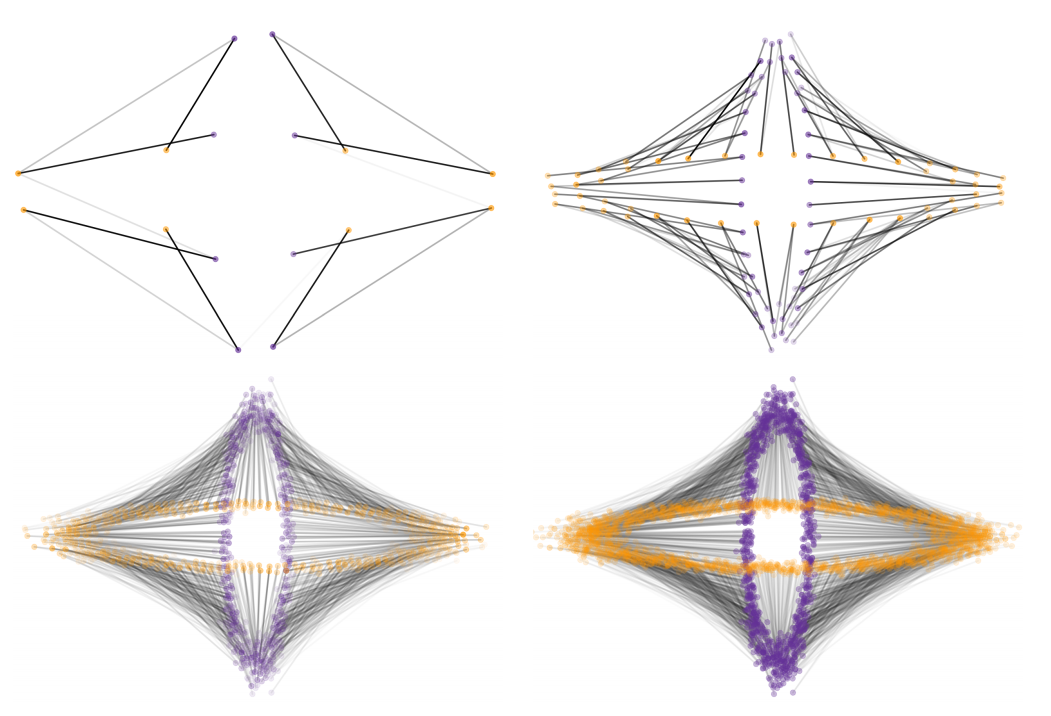
\includegraphics[width=0.6\linewidth]{img/ellipse}
    \label{fig:ot}
    \caption{Illustration of Optimal Transport on Ellipse dataset with different coarsen level}
  \end{figure}

Caffarelli's example consists of two uniform samples on $[-1, 1]^2$ of size $n$. Any points outside the unit circle are then
discarded. Additionally, the target data sample is split along the x-Axis at $0$ and shifted by
$+2$ and $-2$ for points with positive and negative x-Axis values, respectively.

\begin{figure}[htbp]
    \centering
    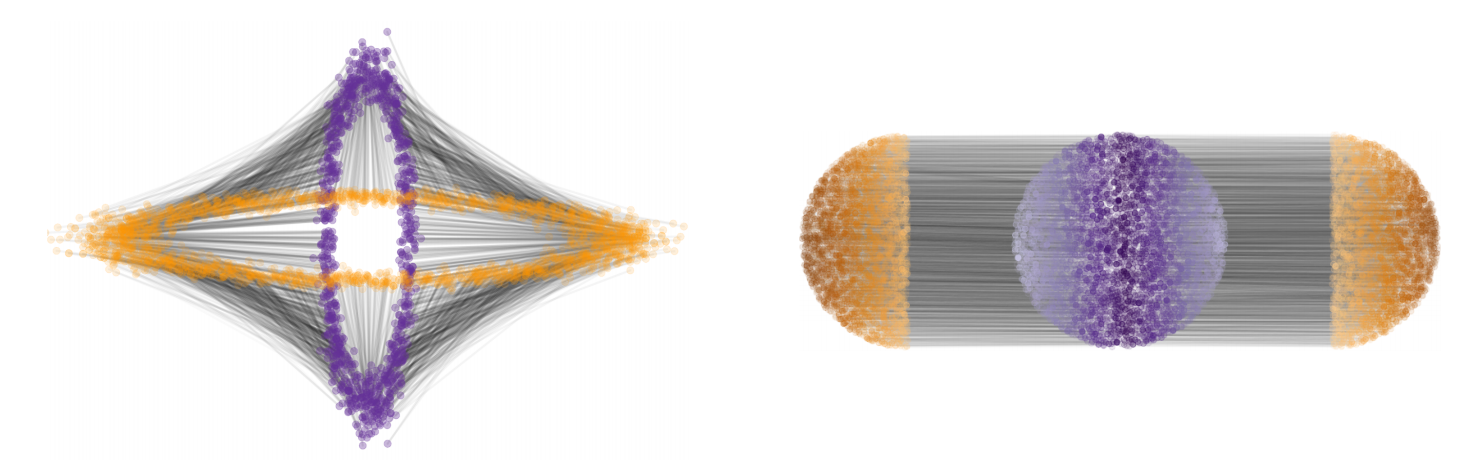
\includegraphics[width=0.6\linewidth]{img/ellipse_caffa}
    \label{fig:ot}
    \caption{Illustration of Optimal Transport on Ellipse dataset and Caffarelli dataset}
  \end{figure}

The DOT benchmark [6] consists of 10 classes of 10 different images, each of which is available at the 5 different
resolutions from $a \times a  = 32 \times 32$ to $512 \times 512$. In computation, each data point is $m = n = a^2$.  This allows
for a total of 45 computations of Wasserstein distances between two images for any one class at any fixed resolution. for convenience, we used the $32 \times 32$ and $64 \times 64$ smaples for experiments.

Table 1 gives an overview of how the classes were created.
Classes 1-7 are random simulations of scenarios based on various probability distributions.
Images at different resolutions are generated independently from each other but according to the same laws.
Classes 8-10 were obtained by ad-hoc choices of simple geometric shapes, classic test images and images of mitochondria acquired using STED
super-resolution microscopy. For geometric shapes and classic test images
the various resolutions available are coarsenings of a single image. For the microscopy
images different clippings of various sizes have been selected from larger images to obtain
the various resolutions.

\vspace{5ex}
\begin{table}[htbp]
	\caption{DOTmark datasent}
	\centering
	\begin{tabular}[width=1.0\linewidth]{lll}
		\toprule
		\quad  & Dataset & Description\\
    \midrule
            1  & WhiteNoise    & i.i.d. uniformly distributed values in [0, 1] at each pixel\\
            2  & GRFrough      & GRF with $\sigma = 1$, $\nu = 0.25$, $\gamma = 0.5$\\
            3  & GRFmoderate   & GRF with $\sigma = 1$, $\nu = 2.5$, $\gamma = 0.15$\\
            4  & GRFsmooth     & GRF with $\sigma = 1$, $\nu = 2.5$, $\gamma = 0.3$\\
            5  & LogGRF        & exp-function of a GRF with $\sigma = 1$, $\nu = 0.5$, $\gamma = 0.4$\\
            6  & CauchyDensity & Bivariate Cauchy density with random center and a varying scale ellipse\\
            7  & LogitGRF      & Logistic function of a GRF with $\sigma = 4$, $\nu = 4.5$, $\gamma = 0.1$\\
            8  & Shapes        & An ad-hoc choice of simple geometric shapes\\
            9  & ClassicImages & Standard grayscale test images used in image processing\\
            10 & Microscopy    & Clippings from STED microscopy images of mitochondria\\
        \bottomrule
	\end{tabular}
	\label{tab:tabledot}
\end{table}

\begin{figure}[htbp]
    \centering
    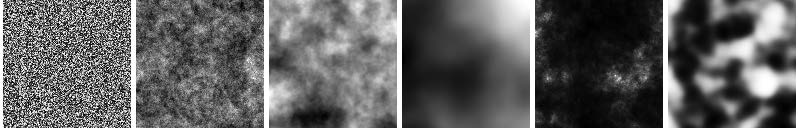
\includegraphics[width=0.9\linewidth]{img/dot_1to6}
    \label{fig:ot}
    \caption{The images in the classes 1-6 at resolution 128 $\times$ 128}
\end{figure}

\begin{figure}[htbp]
    \centering
    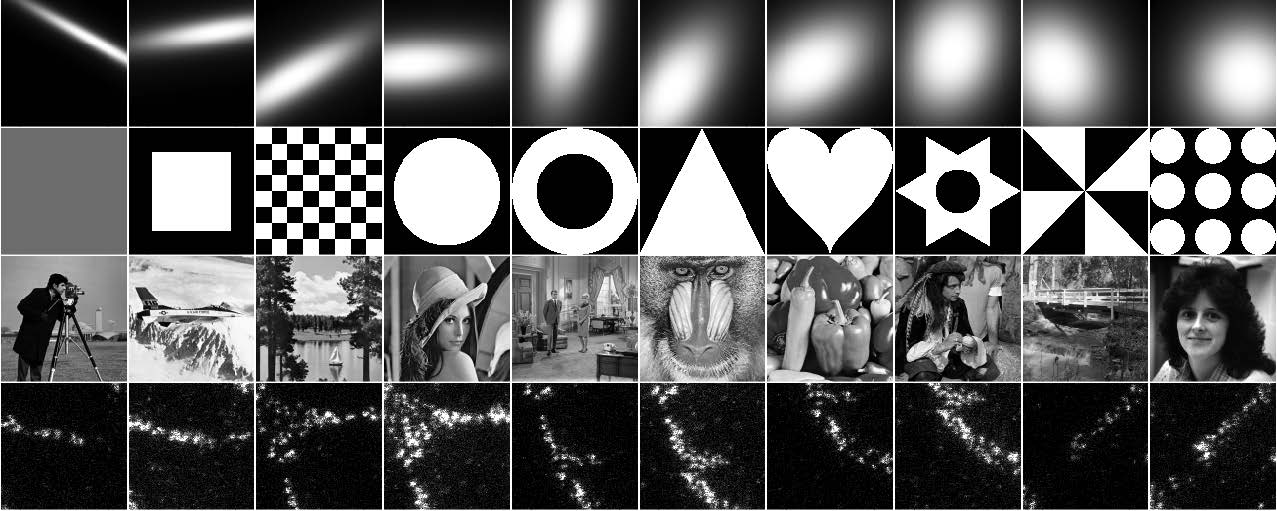
\includegraphics[width=0.9\linewidth]{img/dot_7to10}
    \label{fig:ot}
    \caption{The images in the classes 7-10 at resolution 128 $\times$ 128}
\end{figure}

\clearpage
\subsection{Numercial Results and Intepretations}

We use three main metrics to evaluate all of these algorithms:

\begin{itemize}
    \item Running time
    \item Function value
    \item Constraints $\mu$ and $\nu$ 
\end{itemize}

To measure the satisfaction of constraints, $\mathbf{L}_1$ norm of $\mathbf{\mu} - \mathbf{\pi}_{i\cdot}$ and $\mathbf{\nu} - \mathbf{\pi}_{\cdot j}$ was introduced. On the consideration of time consuming, we conduct our experiments with size $m = n = 64, 128, 256, 512, 1024, 2048$.

Obviously, the running time is an important metrics to measure different algorithms under different test data. In addition, object value can also shows performance of different algorithms, though for entropy regularized methods such as sinkhorn algorithm the function value has been modified with regularization term and then can not be use for comparison.
However, the distance between the suboptimal tranport variable $\pi$ and the optimal transport variable $\tilde \pi$ does not reflect the merits of the algorithm, because it depends on the nature of the cost matrix $\mathbf{C}$. Consider the following example:

\begin{equation}
    \begin{array}{cl}
        {\min } & {\mathbf{t} \mathbf{r}\left(\left(\begin{array}{cc}
        {1+\epsilon} & {1 + \frac{\epsilon}{2}}\\
        {1} & {1} \\
        \end{array}\right)\left(\begin{array}{cc}
        {\pi_{11}} & {\pi_{12}} \\
        {\pi_{21}} & {\pi_{22}}
        \end{array}\right)\right.} \\
        {\text { s.t. }} & {\pi_{11}+\pi_{12}=1} \\
        & {\pi_{21}+\pi_{22}=1} \\
        & {\pi_{11}+\pi_{21}=1} \\
        & {\pi_{12}+\pi_{22}=1}
    \end{array}
\end{equation}

Then the difference between the object value of the optimal solution $\tilde \pi_{ij} = \left(\begin{array}{ll}{0} & {1} \\{1} & {0}\end{array}\right)$ and the suboptimal solution $\pi = \left(\begin{array}{ll}{1} & {0} \\{0} & {1}\end{array}\right)$ is less than $\epsilon$, but the distance after the two are transformed into a vector is significantly larger than $\epsilon$.

Tables below show our experiments results, more detailed data can be found in \textbf{/code/results} folder.

\begin{table}[htbp]
	\caption{Results of Raw Mosek solver and Raw Gurobi solver on Random Generated Dataset}
	\centering
    \begin{tabular}{|c|c|llllll|}
    \hline
    $m = n$             &          & Mosek primal & Mosek dual  & Mosek interior & Gurobi primal & Gurobi dual & Gurobi interior\\
    \hline
    \multirow{4}*{64}   &err $\mu$ & 1.73472e-17  & 1.56125e-17 & 6.99572e-11    & 1.56125e-17   & 1.90820e-17 & 1.56125e-17    \\   
                        &err $\nu$ & 1.73472e-16  & 1.68268e-16 & 6.05657e-11    & 1.56125e-16   & 1.58727e-16 & 1.54390e-16    \\  
                        &fval      & 2.07168e-02  & 2.07168e-02 & 2.07168e-02    & 2.07168e-02   & 2.07168e-02 & 2.07168e-02    \\
                        &time      & 3.12448e-02  & 3.47526e-02 & 3.42710e-02    & 4.78537e-02   & 4.80292e-02 & 7.72452e-02    \\
    \hline
    \multirow{4}*{128}  &err $\mu$ & 7.38910e-06  & 1.04083e-17 & 6.21169e-12    & 3.46945e-18   & 3.46945e-18 & 5.20417e-18    \\   
                        &err $\nu$ & 7.38910e-06  & 1.14275e-16 & 6.21459e-12    & 1.18395e-16   & 1.18395e-16 & 1.17934e-16    \\  
                        &fval      & 1.85776e-02  & 1.85775e-02 & 1.85775e-02    & 1.85775e-02   & 1.85775e-02 & 1.85775e-02    \\
                        &time      & 8.82461e-02  & 1.05152e-01 & 3.42710e-02    & 2.18717e-01   & 2.67161e-01 & 3.70859e-01    \\
    \hline
    \multirow{4}*{256}  &err $\mu$ & 1.75611e-05  & 3.62395e-17 & 8.84693e-11    & 1.04083e-17   & 1.12757e-17 & 1.12757e-17    \\   
                        &err $\nu$ & 1.75611e-05  & 3.43123e-16 & 8.84696e-11    & 3.23526e-16   & 3.23526e-16 & 3.23960e-16    \\  
                        &fval      & 9.37655e-03  & 9.37637e-03 & 9.37637e-03    & 9.37637e-03   & 9.37637e-03 & 9.37637e-03    \\
                        &time      & 3.19547e-01  & 4.38276e-01 & 5.48973e-01    & 1.01217e+00   & 1.12126e+00 & 1.07492e+00    \\
    \hline
    \multirow{4}*{512}  &err $\mu$ & 4.29996e-05  & 5.06695e-17 & 1.13676e-10    & 8.48388e-18   & 3.10109e-16 & 1.12757e-17    \\   
                        &err $\nu$ & 4.29996e-05  & 3.38688e-16 & 1.13677e-10    & 8.48388e-18   & 1.25767e-17 & 3.23960e-16    \\  
                        &fval      & 4.30472e-03  & 4.30454e-03 & 4.30454e-03    & 4.30454e-03   & 4.30454e-03 & 9.37637e-03    \\
                        &time      & 1.42172e+00  & 2.23522e+00 & 2.73145e+00    & 3.47143e+00   & 3.77973e+00 & 1.07492e+00    \\
    \hline    
    \multirow{4}*{1024} &err $\mu$ & 1.06018e-04  & 1.47138e-16 & 1.01099e-13    & 1.09504e-17   & 3.64400e-16 & 1.20346e-17    \\   
                        &err $\nu$ & 1.06018e-04  & 5.08930e-16 & 1.00871e-13    & 3.64753e-16   & 1.15196e-17 & 3.65837e-16    \\  
                        &fval      & 1.94602e-03  & 1.94578e-03 & 1.94578e-03    & 1.94578e-03   & 1.94578e-03 & 1.94578e-03   \\
                        &time      & 6.45907e+00  & 1.37058e+01 & 1.33225e+01    & 1.73826e+01   & 1.31655e+01 & 1.73745e+01    \\
    \hline
    \multirow{4}*{2048} &err $\mu$ & 2.65157e-04  & 1.12464e-16 & 5.64365e-11    & 1.20889e-17   & 9.78113e-16 & 1.13841e-17    \\   
                        &err $\nu$ & 2.65157e-04  & 1.08728e-15 & 5.36207e-11    & 9.76758e-16   & 9.18861e-18 & 9.75701e-16    \\  
                        &fval      & 1.50347e-03  & 1.50297e-03 & 1.50297e-03    & 1.50297e-03   & 1.50297e-03 & 1.50297e-03   \\
                        &time      & 3.59507e+01  & 1.28866e+02 & 6.74333e+01    & 3.16742e+01   & 5.92715e+01 & 9.67955e+01    \\
    \hline   
    \end{tabular}
    \label{tab:table1}
\end{table}

It seems that Gurobi can always reach the real optimal solution, and MOSEK sometimes fails. For MOSEK,
 the simplex method on primal problem is faster than the interior method and dual simplex method. For Gurobi, the simplex method is usually faster than the interior method. As one of the most famous algorithms in 20th century, simplex method was designed for solving linear programming problems. Poor performance of dual simplex may be caused by a large number of constraints. In summary, Gurobi has better performance that MOSEK.

\begin{table}[htbp]
	\caption{Results of ADMM, Sinkhorn and BlockCA algorithm on Random Generated Dataset}
	\centering
    \begin{tabular}{|c|c|lllll|}
    \hline
    $m = n$             &          & Gurobi primal & ADMM primal & ADMM dual   & Sinkhorn    & BlockCA    \\
    \hline
    \multirow{4}*{64}   &err $\mu$ & 1.56125e-17   & 1.40712e-05 & 6.50195e-01 & 1.00180e-16 & 5.41017e-16\\   
                        &err $\nu$ & 1.56125e-16   & 1.41582e-05 & 6.27594e-01 & 1.90874e-16 & 3.94243e-16\\  
                        &fval      & 2.07168e-02   & 2.07460e-02 & 8.77846e-04 & 2.73941e-02 & 2.73941e-02\\
                        &time      & 4.78537e-02   & 1.22792e+00 & 1.38214e+00 & 8.93044e-03 & 1.44658e-01\\
    \hline
    \multirow{4}*{128}  &err $\mu$ & 3.46945e-18   & 4.72795e-05 & 8.45667e-01 & 1.39456e-16 & 5.54624e-16\\   
                        &err $\nu$ & 1.18395e-16   & 4.64422e-05 & 8.56649e-01 & 2.61211e-16 & 5.22084e-16\\  
                        &fval      & 1.85775e-02   & 1.85941e-02 & 8.22017e-05 & 2.92237e-02 & 2.92237e-02\\
                        &time      & 2.67161e-01   & 4.53466e+00 & 3.89032e+00 & 6.39679e-02 & 4.98657e-01\\
    \hline
    \multirow{4}*{256}  &err $\mu$ & 1.04083e-17   & 4.96761e-05 & 9.04781e-01 & 3.11044e-16 & 6.12256e-16\\  
                        &err $\nu$ & 3.23526e-16   & 5.02865e-05 & 9.00866e-01 & 3.62530e-16 & 5.78530e-16\\ 
                        &fval      & 9.37637e-03   & 9.38144e-03 & 1.20866e-05 & 2.88136e-02 & 2.88136e-02\\
                        &time      & 1.01217e+00   & 1.81699e+01 & 8.70793e+00 & 8.24754e-02 & 2.26562e+00\\
    \hline
    \multirow{4}*{512}  &err $\mu$ & 8.48388e-18   & 1.31110e-04 & 9.53515e-01 & 3.42523e-16 & 6.55963e-16\\   
                        &err $\nu$ & 8.48388e-18   & 1.33937e-04 & 9.53115e-01 & 5.30280e-16 & 7.73707e-16\\  
                        &fval      & 4.30454e-03   & 4.30575e-03 & 1.35802e-06 & 2.81078e-02 & 2.81078e-02\\
                        &time      & 3.47143e+00   & 7.43271e+01 & 6.13705e+01 & 2.81078e-01 & 1.08770e+01\\
    \hline    
    \multirow{4}*{1024} &err $\mu$ & 1.09504e-17   & 2.73918e-04 & 9.72007e-01 & 3.86662e-16 & 6.89612e-16\\   
                        &err $\nu$ & 3.64753e-16   & 2.74108e-04 & 9.72809e-01 & 7.61287e-16 & 1.02598e-15\\ 
                        &fval      & 1.94578e-03   & 1.94916e-03 & 2.51372e-07 & 2.79386e-03 & 2.79386e-02\\
                        &time      & 1.73826e+01   & 3.67489e+02 & 2.08239e+02 & 1.02975e+00 & 3.62734e+01\\
    \hline
    \multirow{4}*{2048} &err $\mu$ & 1.20889e-17   & 1.01361e-03 & 9.88752e-01 & 9.68066e-16 & 1.09343e-15\\   
                        &err $\nu$ & 9.76758e-16   & 1.02573e-03 & 9.89591e-01 & 1.09554e-15 & 1.53059e-15\\  
                        &fval      & 1.50297e-03   & 1.49998e-03 & 2.11058e-08 & 2.76252e-03 & 2.76252e-02\\
                        &time      & 3.16742e+01   & 5.71285e+03 & 3.14300e+03 & 8.98797e+00 & 4.12741e+02\\
    \hline
    \end{tabular}
    \label{tab:table1}
\end{table}

Generally speaking, The ADMM method does not have good performance. On the one hand, the error term is large, which is because the equality constraint is difficult to achieve. On the other hand, the required time is much longer than the general algorithm of Mosek and Gurobi. This is because the algorithm will stay at $\pi = \frac{1}{m n}$ for a long time, and it will not start the convergence step until some variables start to increase significantly. what's more, ADMM method is a first order method which means it has slow convergence rate.

As mentioned before, in practice, the Sinkhorn algorithm suffers from numerical overflow when the regularization parameter $\epsilon$ is small compared to the entries of the cost
matrix $\mathbf{C}$. This concern can be alleviated to some extent by carrying out computations
in the log domain. Here Block Coordinate Ascent algorithm was introduced. From the experiments we can see that entropy regularized methods applied with Sinkhorn algorithm and Block Coordinate Ascent algorithm convergence very fast with the slightest violation with all the constraints of $\mu$ and $\nu$ corresponding to err $\mu$ and err $\nu$ shown.

 \begin{table}[htbp]
	\caption{Results of Raw Mosek solver and Raw Gurobi solver on DOTmark Dataset}
	\centering
    \begin{tabular}{|c|c|llllll|}
    \hline
    Class                   &          & Mosek primal & Mosek dual  & Mosek interior & Gurobi primal & Gurobi dual & Gurobi interior\\
    \hline
    \multirow{4}*{WNoise}   &err $\mu$ & 1.04105e-04  & 1.43060e-16 & 2.60955e-11    & 0.00000e+00   & 0.00000e+00 & 0.00000e+00    \\   
                            &err $\nu$ & 1.04106e-04  & 6.93859e-10 & 7.19976e-10    & 6.93859e-10   & 6.93859e-10 & 6.93859e-10    \\  
                            &fval      & 6.49762e-04  & 6.49817e-04 & 6.49817e-04    & 6.49817e-04   & 6.49817e-04 & 6.49817e-04    \\
                            &time      & 6.37157e+00  & 1.00645e+01 & 1.09153e+01    & 1.96804e+01   & 1.80495e+01 & 2.56732e+01    \\
    \hline
    \multirow{4}*{GRFrough} &err $\mu$ & 9.86331e-05  & 2.14455e-16 & 3.88285e-14    & 0.00000e+00   & 0.00000e+00 & 0.00000e+00    \\   
                            &err $\nu$ & 9.86322e-05  & 8.99345e-10 & 8.99386e-10    & 8.99345e-10   & 8.99345e-10 & 8.99345e-10    \\  
                            &fval      & 1.24126e-03  & 1.24131e-03 & 1.24131e-03    & 1.24131e-03   & 1.24131e-03 & 1.24131e-03    \\
                            &time      & 6.22112e+00  & 1.60985e+01 & 1.20426e+01    & 1.70455e+01   & 1.44343e+01 & 2.98131e+01    \\
    \hline
    \multirow{4}*{GRFmid}   &err $\mu$ & 9.82285e-05  & 1.81604e-16 & 5.15640e-11    & 0.00000e+00   & 5.89424e-10 & 5.89424e-10    \\   
                            &err $\nu$ & 9.82291e-05  & 5.89424e-10 & 7.33106e-10    & 5.89424e-10   & 0.00000e+00 & 0.00000e+00    \\  
                            &fval      & 1.29959e-02  & 1.29962e-02 & 1.29962e-02    & 1.29962e-02   & 1.29962e-02 & 1.29962e-02    \\
                            &time      & 7.08524e+00  & 3.11953e+01 & 1.08397e+01    & 1.62867e+01   & 1.74454e+01 & 2.98980e+01    \\
    \hline
    \multirow{4}*{GRFmid2}  &err $\mu$ & 9.78652e-05  & 1.96051e-16 & 2.27771e-12    & 0.00000e+00   & 4.81123e-10 & 4.81123e-10    \\   
                            &err $\nu$ & 9.78657e-05  & 4.81123e-10 & 4.83410e-10    & 4.81123e-10   & 0.00000e+00 & 0.00000e+00    \\  
                            &fval      & 7.01347e-03  & 7.01329e-03 & 7.01329e-03    & 7.01329e-03   & 7.01329e-03 & 7.01329e-03    \\
                            &time      & 8.29048e+00  & 2.58863e+01 & 1.16190e+01    & 1.54850e+01   & 1.46085e+01 & 1.82575e+01    \\
    \hline    
    \multirow{4}*{LogGRF}   &err $\mu$ & 9.79684e-05  & 1.74543e-16 & 1.41349e-13    & 0.00000e+00   & 0.00000e+00 & 0.00000e+00    \\   
                            &err $\nu$ & 9.79684e-05  & 3.44473e-11 & 3.45826e-11    & 3.44471e-11   & 3.44471e-11 & 3.44471e-11    \\  
                            &fval      & 1.14762e-02  & 1.14762e-02 & 1.14762e-02    & 3.44471e-11   & 1.14762e-02 & 1.14762e-02    \\
                            &time      & 6.61064e+00  & 2.25776e+01 & 1.25897e+01    & 1.46135e+01   & 1.81754e+01 & 2.23398e+01    \\
    \hline
    \multirow{4}*{Cauchy}   &err $\mu$ & 8.95380e-05  & 1.69054e-16 & 4.53139e-11    & 0.00000e+00   & 6.45741e-10 & 6.45741e-10    \\   
                            &err $\nu$ & 8.95387e-05  & 6.45741e-10 & 5.36207e-11    & 6.45741e-10   & 0.00000e+00 & 0.00000e+00    \\  
                            &fval      & 2.70715e-02  & 2.70716e-02 & 2.70716e-02    & 2.70716e-02   & 2.70716e-02 & 2.70716e-02    \\
                            &time      & 6.27543e+00  & 3.43761e+01 & 1.25938e+01    & 1.41227e+01   & 1.66956e+01 & 4.97750e+01    \\
    \hline   
    \multirow{4}*{LogitGRF} &err $\mu$ & 1.04014e-04  & 1.61844e-16 & 6.22315e-10    & 0.00000e+00   & 1.23453e-09 & 1.23453e-09    \\   
                            &err $\nu$ & 1.04013e-04  & 1.23453e-09 & 1.83005e-09    & 1.23453e-09   & 0.00000e+00 & 0.00000e+00    \\  
                            &fval      & 1.90306e-02  & 1.90301e-02 & 1.90301e-02    & 1.90301e-02   & 1.90301e-02 & 1.90301e-02    \\
                            &time      & 6.59682e+00  & 2.55476e+01 & 1.09550e+01    & 1.51339e+01   & 1.87915e+01 & 3.24828e+01    \\
    \hline
    \multirow{4}*{Shape}    &err $\mu$ & 3.10808e-05  & 6.51926e-09 & 1.54226e-08    & 0.00000e+00   & 6.51926e-09 & 6.51926e-09    \\   
                            &err $\nu$ & 3.10743e-05  & 4.77049e-17 & 1.07581e-08    & 6.51926e-09   & 0.00000e+00 & 0.00000e+00    \\  
                            &fval      & 6.00170e-03  & 6.00148e-03 & 6.00148e-03    & 6.00148e-03   & 6.00148e-03 & 6.00148e-03    \\
                            &time      & 2.45428e+00  & 4.44892e+00 & 2.97079e+00    & 1.17216e+01   & 1.16747e+01 & 1.31421e+01    \\
    \hline
    \multirow{4}*{Classic}  &err $\mu$ & 9.68013e-05  & 1.20292e-16 & 8.39560e-12    & 0.00000e+00   & 2.61934e-10 & 2.61934e-10    \\   
                            &err $\nu$ & 9.68016e-05  & 2.61935e-10 & 2.70569e-10    & 2.61934e-10   & 0.00000e+00 & 0.00000e+00    \\  
                            &fval      & 2.13840e-03  & 2.13855e-03 & 2.13855e-03    & 2.13855e-03   & 2.13855e-03 & 2.13855e-03    \\
                            &time      & 7.26325e+00  & 1.91323e+01 & 1.30328e+01    & 1.54186e+01   & 1.40239e+01 & 2.08600e+01    \\
    \hline
    \multirow{4}*{Micro}    &err $\mu$ & 9.11961e-05  & 1.09938e-16 & 1.40660e-10    & 0.00000e+00   & 0.00000e+00 & 0.00000e+00   \\   
                            &err $\nu$ & 9.11973e-05  & 1.25146e-09 & 1.24353e-09    & 1.25146e-09   & 1.25146e-09 & 1.25146e-09    \\  
                            &fval      & 5.60394e-02  & 5.60383e-02 & 5.60383e-02    & 5.60383e-02   & 5.60383e-02 & 5.60383e-02    \\
                            &time      & 5.27145e+00  & 2.11592e+01 & 9.32959e+00    & 1.44868e+01   & 1.58690e+01 & 1.78717e+02    \\
    \hline
    \end{tabular}
    \label{tab:table1}
\end{table}



\begin{table}[htbp]
	\caption{Results of ADMM, Sinkhorn and BlockCA algorithm on DOTmark Dataset}
	\centering
    \begin{tabular}{|c|c|lllll|}
    \hline
    Class                   &          & Gurobi primal & ADMM primal & ADMM dual  & Sinkhorn   & BlockCA    \\
    \hline
    \multirow{4}*{WNoise}   &err $\mu$ & 0.00000e+00   & 1.28341e-04  & 3.33216e-01 & 6.93859e-10 & 1.24606e-07 \\   
                            &err $\nu$ & 6.93859e-10   & 1.16042e-04  & 3.33214e-01 & 7.56495e-16 & 1.27072e-07 \\  
                            &fval      & 6.49817e-04   & 6.49518e-04  & 0.00000e+00 & 2.76750e-03 & 2.76750e-02 \\
                            &time      & 1.96804e+01   & 2.05072e+02  & 1.76776e+02 & 4.96325e-01 & 4.06536e+01 \\
    \hline
    \multirow{4}*{GRFrough} &err $\mu$ & 0.00000e+00   & 1.36891e-04  & 2.13545e-01 & 8.99345e-10 & 1.23457e-07 \\   
                            &err $\nu$ & 8.99345e-10   & 1.35197e-04  & 2.13544e-01 & 7.54279e-16 & 1.22399e-07 \\  
                            &fval      & 1.24131e-03   & 1.24030e-03  & 0.00000e+00 & 2.77295e-02 & 2.77295e-01 \\ 
                            &time      & 1.70455e+01   & 3.08484e+02  & 2.03046e+02 & 5.94349e-01 & 4.29790e+01 \\ 
    \hline
    \multirow{4}*{GRFmid}   &err $\mu$ & 0.00000e+00   & 1.51246e-04  & 2.28186e-01 & 4.81123e-10 & 1.20229e-07 \\    
                            &err $\nu$ & 5.89424e-10   & 1.43893e-04  & 2.28171e-01 & 7.92382e-16 & 1.17900e-07 \\   
                            &fval      & 1.29962e-02   & 1.29985e-02  & 0.00000e+00 & 2.67600e-02 & 2.70585e-02 \\ 
                            &time      & 1.62867e+01   & 3.04346e+02  & 2.04500e+02 & 6.11465e-01 & 3.94406e+01 \\ 
    \hline
    \multirow{4}*{GRFmid2}  &err $\mu$ & 0.00000e+00   & 1.32336e-04  & 1.90867e-01 & 5.89424e-10 & 1.25930e-07 \\    
                            &err $\nu$ & 4.81123e-10   & 1.32346e-04  & 1.90878e-01 & 7.83878e-16 & 1.22960e-07 \\   
                            &fval      & 7.01329e-03   & 7.01429e-03  & 0.00000e+00 & 2.70585e-02 & 2.67600e-01 \\
                            &time      & 1.54850e+01   & 2.56570e+02  & 1.77548e+02 & 5.40904e-01 & 3.97170e+01 \\
    \hline    
    \multirow{4}*{LogGRF}   &err $\mu$ & 0.00000e+00   & 1.55836e-04  & 3.63980e-01 & 3.44471e-11 & 1.28669e-07 \\   
                            &err $\nu$ & 3.44471e-11   & 1.46725e-04  & 3.63993e-01 & 8.62698e-16 & 1.28669e-07 \\  
                            &fval      & 3.44471e-11   & 1.14813e-02  & 0.00000e+00 & 2.25891e-02 & 2.25891e-02\\
                            &time      & 1.46135e+01   & 2.46276e+02  & 1.92535e+02 & 6.65159e-01 & 6.66666e66 \\
    \hline
    \multirow{4}*{Cauchy}   &err $\mu$ & 0.00000e+00   & 2.44488e-04 & 4.14467e-01 & 6.45741e-10 & 1.21786e-07 \\   
                            &err $\nu$ & 6.45741e-10   & 2.03140e-04 & 4.14312e-01 & 8.02487e-16 & 1.32475e-07 \\ 
                            &fval      & 2.70716e-02   & 2.70958e-02 & 0.00000e+00 & 2.07987e-02 & 2.07987e-01 \\
                            &time      & 1.41227e+01   & 3.26161e+02 & 2.28633e+02 & 4.73294e-01 & 3.97828e+01 \\
    \hline   
    \multirow{4}*{LogitGRF} &err $\mu$ & 0.00000e+00   & 1.52596e-04  & 3.99687e-01  & 1.23453e-09 & 1.24918e-07 \\   
                            &err $\nu$ & 1.23453e-09   & 1.43546e-04  & 3.99684e-01  & 8.23705e-16 & 1.26019e-07 \\ 
                            &fval      & 1.90301e-02   & 1.90381e-02  & 0.00000e+00  & 2.81800e-02 & 2.81800e-02 \\
                            &time      & 1.51339e+01   & 2.39396e+02  & 1.36987e+02  & 5.37684e-01 & 3.92088e+01 \\
    \hline
    \multirow{4}*{Shape}    &err $\mu$ & 0.00000e+00   & 1.85553e-04  & 3.60264e-01  & 6.51926e-09 & 4.34572e-08 \\   
                            &err $\nu$ & 6.51926e-09   & 2.04018e-04  & 3.59738e-01  & 5.09141e-16 & 4.54084e-08 \\  
                            &fval      & 6.00148e-03   & 6.00026e-03  & 0.00000e+00  & 1.45999e-02 & 1.45999e-02 \\
                            &time      & 1.17216e+01   & 2.02916e+02  & 1.35861e+02  & 5.54126e-01 & 3.13619e+01 \\
    \hline
    \multirow{4}*{Classic}  &err $\mu$ & 0.00000e+00   & 2.05559e-04 & 1.79544e-01 & 2.61935e-10 & 1.20315e-07 \\   
                            &err $\nu$ & 2.61934e-10   & 2.05644e-04 & 1.79543e-01 & 7.72765e-16 & 1.17474e-07 \\
                            &fval      & 2.13855e-03   & 2.14597e-03 & 0.00000e+00 & 2.80976e-02 & 2.80976e-01 \\
                            &time      & 1.54186e+01   & 3.57276e+02 & 2.30821e+02 & 4.58951e-01 & 3.80998e+01 \\
    \hline
    \multirow{4}*{Micro}    &err $\mu$ & 0.00000e+00   & 1.49094e-04  & 5.35081e-01 & 1.25146e-09 & 1.29936e-07 \\  
                            &err $\nu$ & 1.25146e-09   & 1.22823e-04  & 5.35094e-01 & 6.58111e-16 & 1.64514e-07 \\  
                            &fval      & 5.60383e-02   & 5.60339e-02  & 0.00000e+00 & 2.80043e-01 & 2.80042e-01 \\
                            &time      & 1.44868e+01   & 2.01784e+02  & 1.38029e+02 & 5.59559e-01 & 3.95853e+01 \\
    \hline
    \end{tabular}
    \label{tab:table1}
\end{table}